%=======================================================
%	PACKAGES AND THEMES
%=======================================================
\documentclass[8pt]{beamer}
\mode<presentation> {
\usepackage{etex}
\usetheme{Boadilla}
\definecolor{navyblue}{rgb}{0.0, 0.0, 0.5}
\definecolor{dkgreen}{rgb}{0,0.6,0}
\definecolor{gray}{RGB}{64, 64, 64}
\definecolor{mauve}{rgb}{0.58,0,0.82}
\usecolortheme[named = navyblue]{structure}
\setbeamercolor{normal text}{fg = gray}
\setbeamercolor{frametitle}{fg = white, bg = navyblue}
\setbeamerfont{framesubtitle}{size = \normalsize}
\setbeamerfont{caption}{size=\footnotesize}
\setbeamercolor{page number in head/foot}{fg = gray}
\setbeamertemplate{footline}%[frame number]
}


\usepackage{graphicx} % Allows including images
\usepackage{booktabs} % Allows the use of \toprule, \midrule and \bottomrule in tables
\usepackage{multicol}
\usepackage[export]{adjustbox}
\usepackage{colortbl}
\usepackage{graphicx} 

\usepackage{tikz}
\usepackage{fancybox}
\usepackage[absolute, overlay]{textpos}
\usepackage{multirow}
\usepackage{siunitx}
\usepackage{tcolorbox}


\usepackage{tikz}
\usepackage{calc}
\newlength{\outerradius}
\newlength{\innerradius}
\setlength{\outerradius}{0.50cm}
\setlength{\innerradius}{0.35cm}

%Damit wir Quellcode nutzen können.
\usepackage{listings}
\lstset{numbers=left,
	numberstyle=\tiny,
	numbersep=5pt,
	breaklines=true,
	showstringspaces=false,
	frame=l ,
	xleftmargin=15pt,
	xrightmargin=15pt,
	basicstyle=\ttfamily\scriptsize,
	stepnumber=1,
	keywordstyle=\color{blue},          % keyword style
  	commentstyle=\color{dkgreen},       % comment style
  	stringstyle=\color{mauve}         % string literal style
}
%Sprache Festelegen
\lstset{language=R}


%=======================================================
%	TITLE PAGE
%=======================================================

\title{\textbf{Network Theories}}

\author{Dr Daniele Rotolo}

\institute
{
SPRU (Science Policy Research Unit) \\
Business School\\
University of Sussex \\

\medskip

\medskip

\medskip

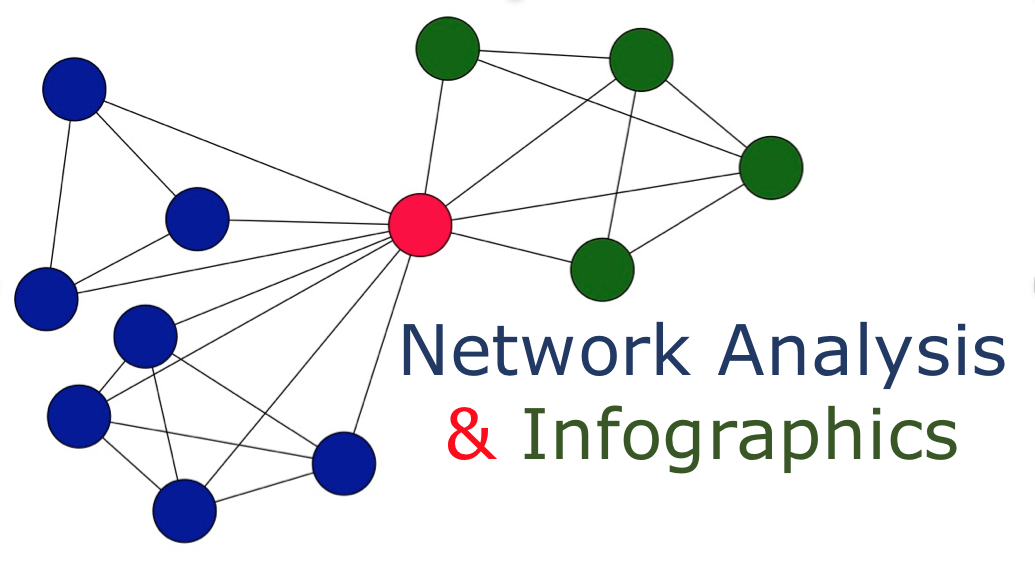
\includegraphics[width=2.5cm]{../_shared_pics/logo}

\medskip

\textit{{\color{dkgreen}{Week 10}}}\\
}


\date{} % Date, can be changed to a custom date

\begin{document}

\begin{frame}
\titlepage % Print the title page as the first slide

\begin{textblock*}{10pt}(0pt, 0.9\textheight)

\includegraphics[width=4cm]{../_shared_pics/SPRU.png}
\end{textblock*}

\end{frame}


%=======================================================
%	Learning outcomes
%=======================================================

\begin{frame}
\frametitle{Learning Outcomes}

\centering
\footnotesize
\begin{tabular}{lp{5.5cm}l}
\toprule
\multicolumn{2}{l}{\textbf{Learning outcome}} & \textbf{Assessment mode}\\
\hline
\\
\rowcolor{green!20}1 & 
Explain the concept of network and list the main network indicators & 
ESS\\
\\
2 & 
Describe and apply the major techniques for the collection of network data and their statistical analysis & ESS, GPN + GWS\\
\\
\rowcolor{green!20}3 & 
Identify the main characteristics of networks by means of network measures  & ESS, GPN + GWS\\
\\
4 &
Employ network analysis techniques to produce network data-based infographics & 
GPN + GWS\\
\\
\bottomrule
\multicolumn{3}{l}{Note: ESS: Essay; GPN: Group Presentation; GWS: Group Written Submission}\\
\end{tabular}

\end{frame}

%------------------------------------------------





%=======================================================
%	Intro slides
%=======================================================
\section*{Overview}
%------------------------------------------------

\begin{frame}
\frametitle{\insertsection}
\tableofcontents[hideallsubsections]
\end{frame}






%=======================================================
% Network theorising
%=======================================================
\section{Network theorising}
%------------------------------------------------


\bgroup
\setbeamercolor{background canvas}{bg = navyblue}
\begin{frame}[plain]{}
\begin{center}
\color{white}{\Huge\insertsection}
\end{center}
\end{frame}
\egroup

%------------------------------------------------



\begin{frame}
\frametitle{\insertsection}

{\color{blue}{Network analysis}} is not a theory \textit{per se}, but it is a methodological tool to support the development of theories \cite{Borgatti2011}

\end{frame}

%------------------------------------------------

\begin{frame}
\frametitle{\insertsection}

\centering
\Large What is a theory?

\end{frame}

%------------------------------------------------

\begin{frame}
\frametitle{\insertsection}
\framesubtitle{What is a theory?}


\begin{columns}[c]
\column{.45\textwidth} 
A {\color{blue}{theory}} can be defined as

\begin{itemize}
\item A set of {\color{blue}{laws}} that are empirically supported
\item A set of interrelated {\color{blue}{definitions}}, {\color{blue}{axioms}}, and {\color{blue}{propositions}}
\item A set of {\color{blue}{descriptions of casual processes}}
\end{itemize}


\column{.45\textwidth}
\centering

\includegraphics[width=0.8\textwidth, frame]{theory}\\
{\tiny\cite{Reynolds1971}}

\end{columns}

\end{frame}


%==NOTE==
% An axiom is a statement which is regarded as being established, accepted, or self-evidently true without proof
%Here is an axiom of addition and multiplication.
%Let x and y be real numbers.
%Then x + y is also a real number and xy is also a real number.
%Euclidean geometry: a line is breadthless length, i.e. it has only one dimension
%A propositions is a statement which is offered up for investigation as to its truth or falsehood
%========




%------------------------------------------------

\begin{frame}
\frametitle{\insertsection}

\centering
\Large Why do we need theories?

\end{frame}

%------------------------------------------------

\begin{frame}
\frametitle{\insertsection}
\framesubtitle{Why do we need theories?}


\cite{Reynolds1971}
\begin{itemize}
\item To {\color{blue}{predict}} the outcomes of processes 
\item To {\color{blue}{explain}} processes (sense of understanding)
\item To {\color{blue}{control}} processes
\end{itemize}


\end{frame}

%------------------------------------------------


\begin{frame}
\frametitle{\insertsection}


\centering
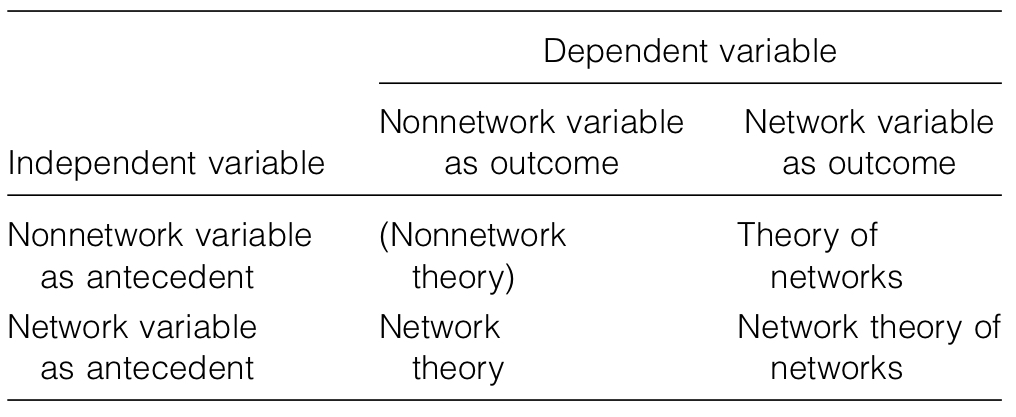
\includegraphics[width=7cm]{borgatti}\\
{\tiny Source: \cite{Borgatti2011}}


\vspace{1cm}

\begin{columns}[t]
\column{.45\textwidth}
\footnotesize
{\color{blue}{Network theory}}\\
Mechanisms and processes that interact with network structures to produce certain outcomes for individuals, groups, and organisations (e.g.\ firms' performance, individuals' creativity)

\column{.45\textwidth} 
\footnotesize
{\color{blue}{Theory of networks}}\\
Mechanisms and processes that explain why networks have certain structures (i.e.\ antecedents of network properties)
\end{columns}

\end{frame}

%------------------------------------------------




%=======================================================
% Social capital theory
%=======================================================
\section{Social capital theory}
%------------------------------------------------

\bgroup
\setbeamercolor{background canvas}{bg = navyblue}
\begin{frame}[plain]{}
\begin{center}
\color{white}{\Huge\insertsection}
\end{center}
\end{frame}
\egroup

%------------------------------------------------

\begin{frame}
\frametitle{\insertsection}


{\color{blue}{Social capital}} is ``the sum of the actual and potential resources embedded within, available through, and derived from the network of relationships possessed by an individual or social unit''\\
\vspace{0.5cm}
\cite{Nahapiet1998}  

\end{frame}

%------------------------------------------------

\begin{frame}
\frametitle{\insertsection}
\framesubtitle{Core idea}

\begin{itemize}
\item Others (e.g.\ friends, acquaintances) tend to have {\color{blue}{goodwill}} towards us
\item This goodwill is a valuable {\color{blue}{resource}}
\item {\color{dkgreen}{Benefits}} and {\color{red}{risks}}
    \begin{itemize}
    \item Access to information (quality, relevance, timeliness)
    \item Influence, control, and power (brokerage opportunities)
    \item Time and resources to establish and maintain relationships
    \item Overembeddedness -- ``the ties that bind can also become the
ties that blind'' \cite{Powell1994}
    \end{itemize}
\end{itemize}
 

\end{frame}

%------------------------------------------------

\begin{frame}
\frametitle{\insertsection}
\framesubtitle{Impact}

Social capital \cite{Adler2002}
\begin{itemize}
\item influences career success and executive compensation
\item supports the job seeking process
\item facilitates the exchange of resources and product innovation in organisations
\item supports the creation of intellectual capital
\item stimulates entrepreneurship and the formation of start-up companies
\item strengthens inter-organisational learning
\item ...
\end{itemize}
 

\end{frame}

%------------------------------------------------

\begin{frame}
\frametitle{\insertsection}

Dimensions of social capital \cite{Nahapiet1998}  

\medskip

\begin{itemize}
\item {\color{blue}{Structural}}: properties of the network of relations
    \begin{itemize}
    \item presence/absence of ties
    \item network-level measures (e.g.\ density)
    \item node-level measures (e.g.\ centrality)
    \end{itemize}

\medskip

\item {\color{blue}{Relational}}: type of relations between individuals 
    \begin{itemize}
    \item friendship
    \item emotional attachment to other actors
    \item trust, obligations, expectations
    \end{itemize}

\medskip

\item {\color{blue}{Cognitive}}
    \begin{itemize}
    \item shared representations
    \item interpretations
    \end{itemize}

\end{itemize} 

\end{frame}

%------------------------------------------------

\begin{frame}
\frametitle{\insertsection}

Within social capital theory
    \begin{itemize}
    \item {\color{blue}{Strength of weak ties (SWT)}} \cite{Granovetter1973}
    \item {\color{blue}{Brokerage and structural holes (SH)}} \cite{Burt1992} 
    \end{itemize}
    
\end{frame}

%------------------------------------------------




%=======================================================
% Strength of weak ties (SWT)
%=======================================================
\section{Strength of weak ties (SWT)}
%------------------------------------------------

\bgroup
\setbeamercolor{background canvas}{bg = navyblue}
\begin{frame}[plain]{}
\begin{center}
\color{white}{\Huge\insertsection}
\end{center}
\end{frame}
\egroup

%------------------------------------------------

\begin{frame}
\frametitle{\insertsection}

\begin{columns}[c]
\column{.45\textwidth} 
{\color{blue}{Strength of weak ties}}\\
An actor's weak ties are more likely to be source of novel information than the actor's stronger ties

\column{.45\textwidth}
\centering
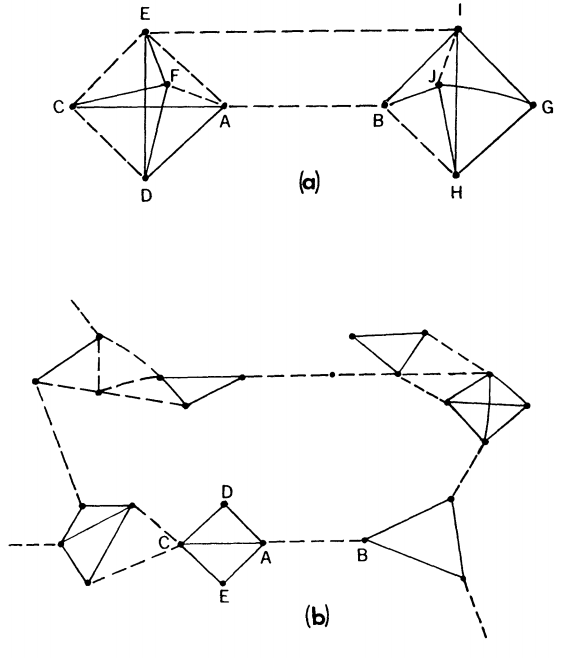
\includegraphics[width=\textwidth]{swt}\\
{\tiny \cite{Granovetter1973}}

\end{columns}

\end{frame}

%------------------------------------------------

\begin{frame}
\frametitle{\insertsection}
\framesubtitle{Rationale}


{\color{blue}{Premise 1}}: The stronger is a tie between two actors the more likely the `social worlds' of these will overlap
    
\begin{itemize}
\item {\color{blue}{Transitivity}}: $A \leftrightarrow B$, $B \leftrightarrow C$ are strong $\Rightarrow A\leftrightarrow C$ is at least weak
\item {\color{blue}{Homophily}}: individuals tend to be homophilous (i.e.\ they establish stronger ties with individuals that are similar to themselves) \cite{McPherson2001}
\end{itemize}

\medskip
\medskip

\centering
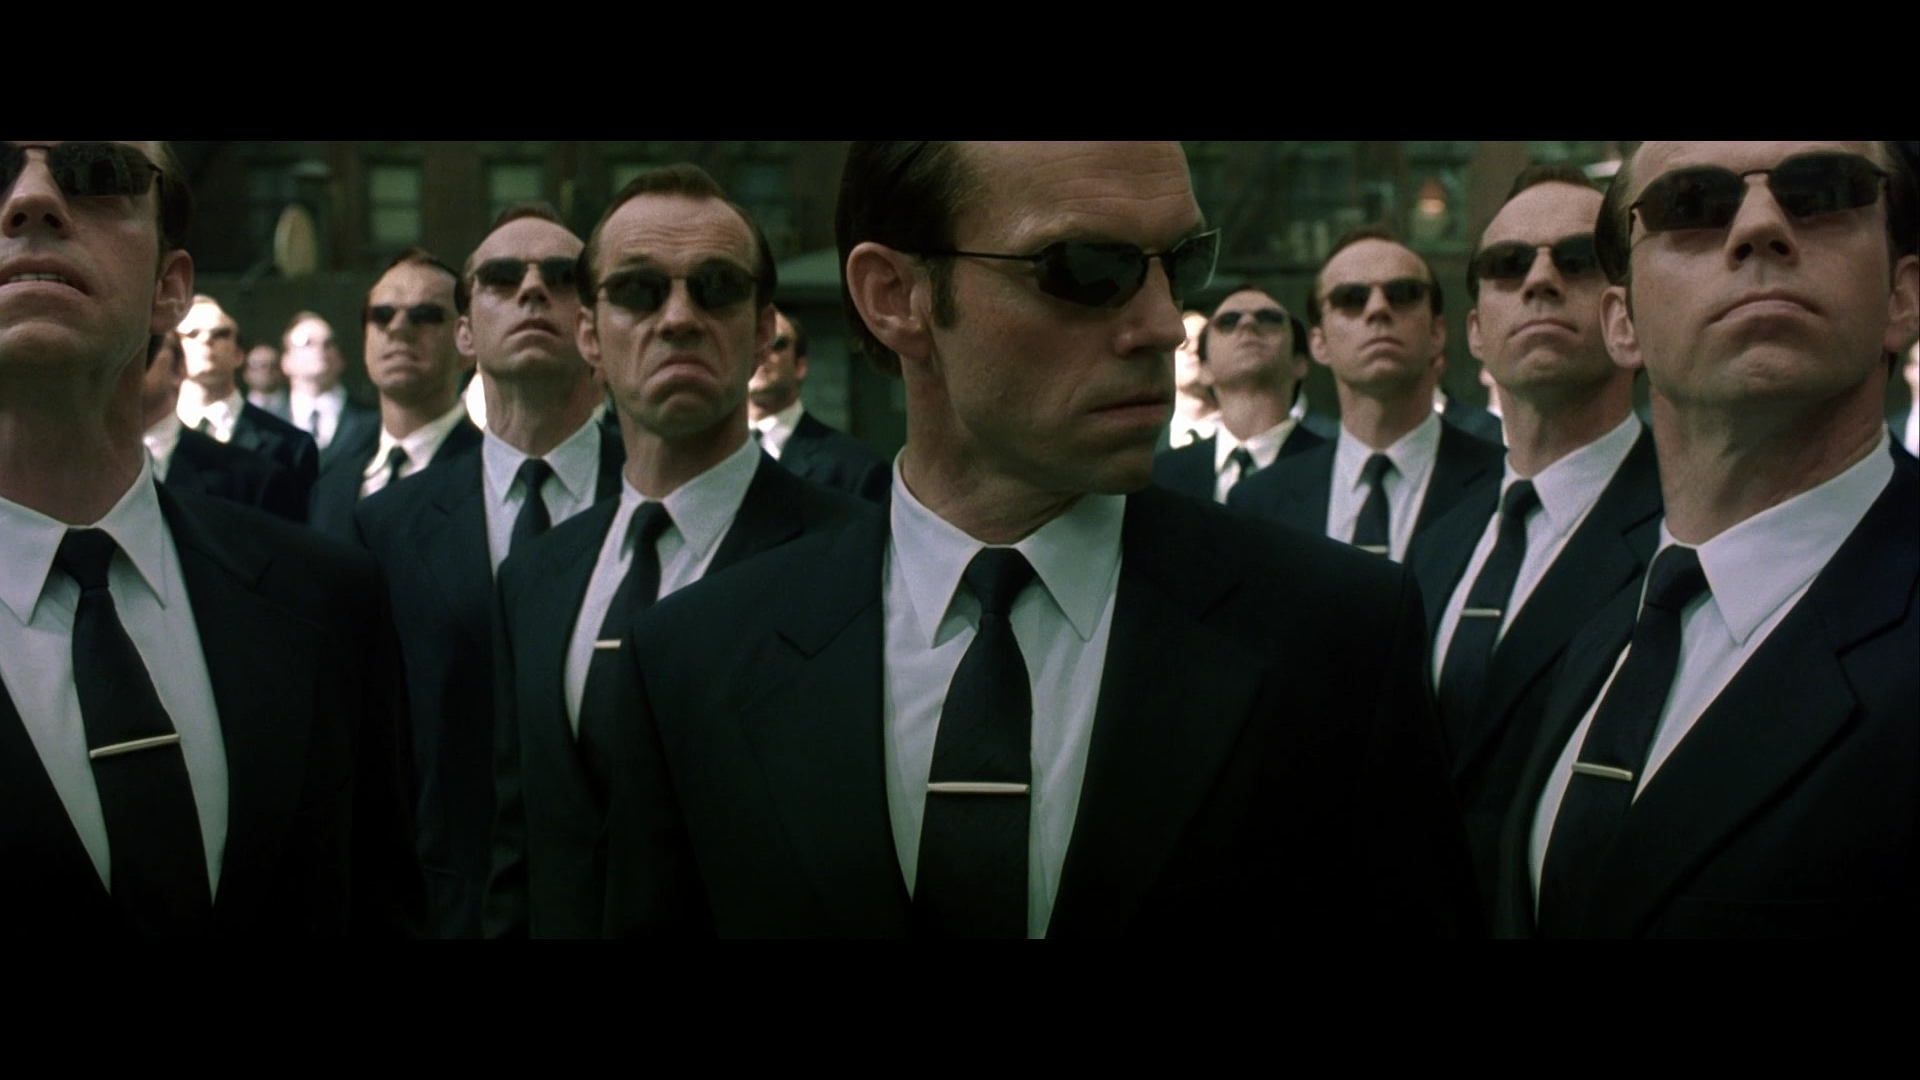
\includegraphics[width=6cm]{homophily}\\
{\tiny Source: Matrix Revolution}

\end{frame}

%------------------------------------------------

\begin{frame}
\frametitle{\insertsection}
\framesubtitle{Rationale}

\begin{columns}[c]
\column{.45\textwidth} 
{\color{blue}{Premise 2}}: Bridging ties are potential sources of novel ideas

\begin{itemize}
\item Bridging ties link individuals not connected through friends
\item Access to information that is not circulating among close contacts
\end{itemize}


\column{.45\textwidth}
\centering
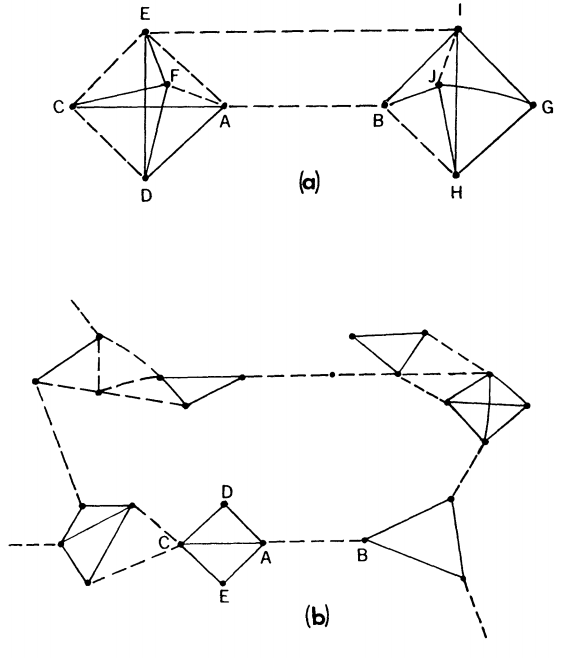
\includegraphics[width=\textwidth]{swt}\\
{\tiny \cite{Granovetter1973}}

\end{columns}

\end{frame}

%------------------------------------------------

\begin{frame}
\frametitle{\insertsection}
\framesubtitle{Rationale}
	
\begin{columns}[c]
\column{.45\textwidth} 
{\color{blue}{Premise 1}} + {\color{blue}{Premise 2}}: Strong ties are unlikely to be source of novelty

\begin{itemize}
\item Bridging ties are unlikely to be strong ties ($A \leftrightarrow B$ is strong, $B\leftrightarrow D$ should be at least weak)
\item Weak ties are more likely to be bridging ties
\item Weak ties are more likely to provide access to novel information
\item \textit{Empirical evidence: weak ties provide better job opportunities}
\end{itemize}

\column{.45\textwidth}
\centering
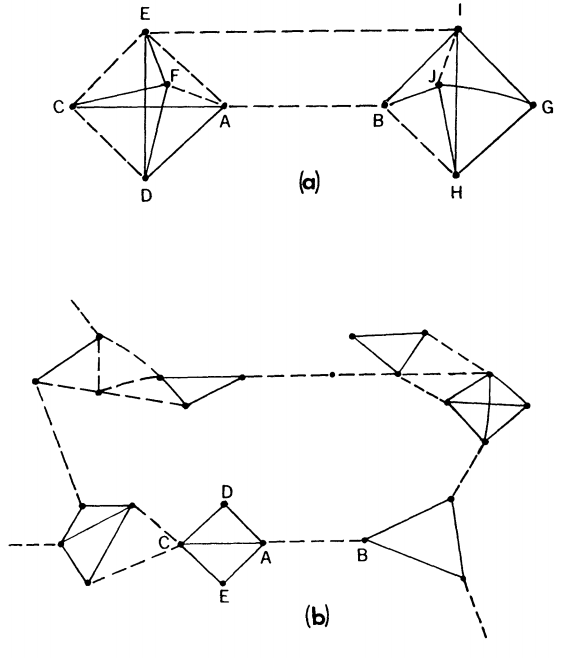
\includegraphics[width=\textwidth]{swt}\\
{\tiny \cite{Granovetter1973}}

\end{columns}	
  


\end{frame}

%------------------------------------------------






%=======================================================
% Structural holes (SH)
%=======================================================
\section{Structural holes (SH)}
%------------------------------------------------

\bgroup
\setbeamercolor{background canvas}{bg = navyblue}
\begin{frame}[plain]{}
\begin{center}
\color{white}{\Huge\insertsection}
\end{center}
\end{frame}
\egroup

%------------------------------------------------

\begin{frame}
\frametitle{\insertsection}

\begin{columns}[c]
\column{.45\textwidth} 
{\color{blue}{Structural holes}}\\
Structural holes in a node's ego network are likely to provide the node with novel information

\medskip
\medskip

\centering
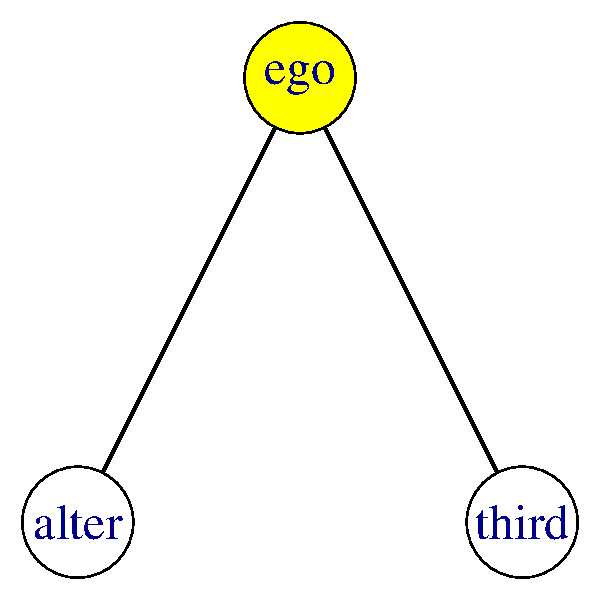
\includegraphics[width=3cm]{opentriad}

\column{.45\textwidth}
\centering

\includegraphics[width=0.8\textwidth]{burtcover}\\
{\tiny \cite{Burt1992}}

\end{columns}

\end{frame}

%------------------------------------------------

\begin{frame}
\frametitle{\insertsection}
\framesubtitle{From Lecture 5}

\begin{columns}
\column{.45\textwidth} 
\begin{itemize}
    \item For each triad we can evaluate the presence of {\color{blue}{structural holes}}
    \item To identify the number of triads we can count the number of possible ties, which is $(N-1)(N-2)/2$ in an undirected network
    \item Example: 6 triads and 5 structural holes
\end{itemize}

\column{.45\textwidth}
\centering
\includegraphics<1>[width=5cm]{base}
\includegraphics<2->[width=5cm]{egonet}
\end{columns}

\end{frame}

%------------------------------------------------

\begin{frame}
\frametitle{\insertsection}
\framesubtitle{From Lecture 6}

\cite{Burt1992} measures of {\color{blue}{brokerage}}

\begin{itemize}
\item Effective Network Size and Efficiency
\item Constraint
\end{itemize}
		
\end{frame}

%------------------------------------------------

\begin{frame}
\frametitle{\insertsection}

\begin{columns}[c]
\column{.45\textwidth} 
\framesubtitle{Rationale}


\begin{itemize}
\item $A$ and $B$ have the same number of ties (degree)
\item $A$ is more likely than $B$ to access novel information (redundancy)
\item As a result, $A$ may perform better than $B$
\end{itemize}


\column{.45\textwidth}
\centering
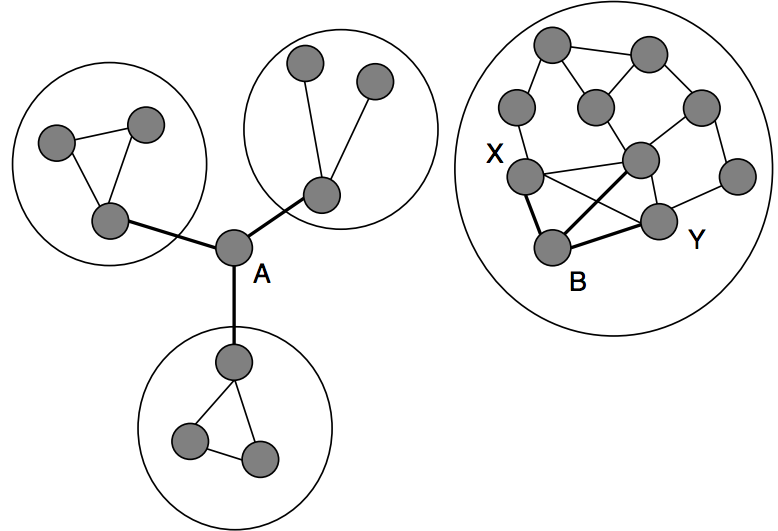
\includegraphics[width=\textwidth]{sh}\\
{\tiny Source: \cite{Borgatti2011}}

\end{columns}

\end{frame}

%------------------------------------------------




%=======================================================
% SWT vs. SH, and other theories
%=======================================================
\section{SWT vs. SH, and other theories}
%------------------------------------------------

\bgroup
\setbeamercolor{background canvas}{bg = navyblue}
\begin{frame}[plain]{}
\begin{center}
\color{white}{\Huge\insertsection}
\end{center}
\end{frame}
\egroup

%------------------------------------------------


\begin{frame}
\frametitle{\insertsection}

\footnotesize
\begin{table}
\begin{tabular}{lp{4cm}|p{4cm}}
\toprule
                        & \textbf{SWT}                            & \textbf{SH}\\
                        & \cite{Granovetter1973}                  & \cite{Burt1992}\\
\hline
\\
{\color{blue}{Assumption}}   & \multicolumn{2}{c}{networks distribute information (flow model)}\\
\\
{\color{blue}{Focus}}        & \multicolumn{2}{c}{networks provide access to novel information}\\
\\
{\color{blue}{Network}}                 & whole network           & ego network\\
& &\\
{\color{blue}{Agency}}                  & serendipitous world in which actors accidentally forms ties     & strategic/instrumental (ego's attributes are neglected)\\
& &\\
{\color{blue}{Mechanisms}}              & tie strength            & tie strength and redundancy\\
& &\\
{\color{blue}{Seminal evidence}}        & getting a job           & getting promoted\\
\bottomrule
\end{tabular}
\end{table}

\end{frame}

%------------------------------------------------


%=======================================================
%	Questions
%=======================================================
\bgroup
\setbeamercolor{background canvas}{bg = orange}
\begin{frame}[plain]{}
\begin{center}
\color{white}{\Huge Questions}
\end{center}
\end{frame}
\egroup




%=======================================================
%	References
%=======================================================
\begin{frame}[allowframebreaks]
\frametitle{References}
\tiny
\bibliographystyle{apalike}
\bibliography{/Users/danielerotolo/Dropbox/References/bibtex_references/library.bib}
\end{frame}
%------------------------------------------------








\end{document}